\chapter{Opis struktury}
\label{chap:struk}

\section{Opis struktury projektu}
W tym rozdziale zostanie przedstawiona struktura projektu, wraz z opisem poszczególnych elementów. Projekt jest podzielony na kilka głównych katalogów, z których każdy pełni określoną funkcję.
Rozdział ten zamknie omówienie klas i ich funkcji w projekcie, co pozwoli na lepsze zrozumienie struktury i organizacji kodu. Skupi się też na wymaganiach do uruchomienia projektu, które są niezbędne do poprawnego działania aplikacji.

\section{Wykorzystane technologie i narzędzia}
Rdzeń systemu został zbudowany w oparciu o język Java, który zapewnił wysoką wydajność i niezawodność działania aplikacji. Interfejs użytkownika został zaimplementowany przy użyciu biblioteki Java Swing, oferującej bogaty zestaw komponentów graficznych.\\

Warstwa danych wykorzystuje następujące technologie:

MySQL jako system zarządzania relacyjną bazą danych

JDBC (Java Database Connectivity) jako interfejs łączący aplikację z bazą danych

Zaawansowane zapytania SQL z optymalizacją pod kątem wydajności\\

Środowisko developerskie obejmowało:

IntelliJ IDEA jako główne środowisko programistyczne

Git jako system kontroli wersji z repozytorium hostowanym na GitHubie

Zintegrowane narzędzia do debugowania i profilowania kodu\\

Cała architektura została zaprojektowana z naciskiem na:

Wydajność połączenia z bazą danych

Przejrzystość interfejsu użytkownika

Łatwość rozszerzania funkcjonalności

Bezpieczeństwo przechowywanych danych

\section{Hierarchia i architektura klas}

Projekt jest zorganizowany w sposób hierarchiczny, gdzie główną klasą jest `Main`, która uruchamia aplikację. Poniżej przedstawiono strukturę klas wraz z ich funkcjami:

\begin{itemize}
    \item \textbf{Warstwa Dostępu do baz danych (Dao):} Ta warstwa odpowiada za komunikację z bazą danych MySQL. Zawiera klasy takie jak `AddUsers`, `ReservationDao`, `HousesDao` itd., które implementują metody do wykonywania operacji CRUD (Create, Read, Update, Delete) na odpowiednich tabelach w bazie danych.
    \item \textbf{Warstwa Prezentacji (GUI):} Ta warstwa jest odpowiedzialna za interakcję z użytkownikiem. Zawiera klasy takie jak `AfterLogin`, `Register`, `MainMenu` itd., które implementują graficzny interfejs użytkownika (GUI) przy użyciu biblioteki Swing. Użytkownik może logować się, rejestrować nowe konto oraz przeglądać dostępne usługi.
    \item \textbf{Warstwa Logiki Biznesowej (Services):} Ta warstwa zawiera klasy, które implementują logikę biznesową aplikacji. Przykładowe klasy to `Lakes`, `Houses`, `FishingRods` itd. Odpowiadają one za przetwarzanie danych i wykonywanie operacji na obiektach reprezentujących rezerwacje, domki i wędki.

\end{itemize}
\clearpage

\subsection{Diagram klas UML} 
Diagram klas (Rys. \ref{fig:uml_diagram}) to wizualna „mapa” projektu.
Przedstawia on relacje między klasami, ich atrybuty i metody. Diagram ten jest kluczowym narzędziem do zrozumienia struktury projektu i jego komponentów. 

\begin{figure}[H]
    \centering
    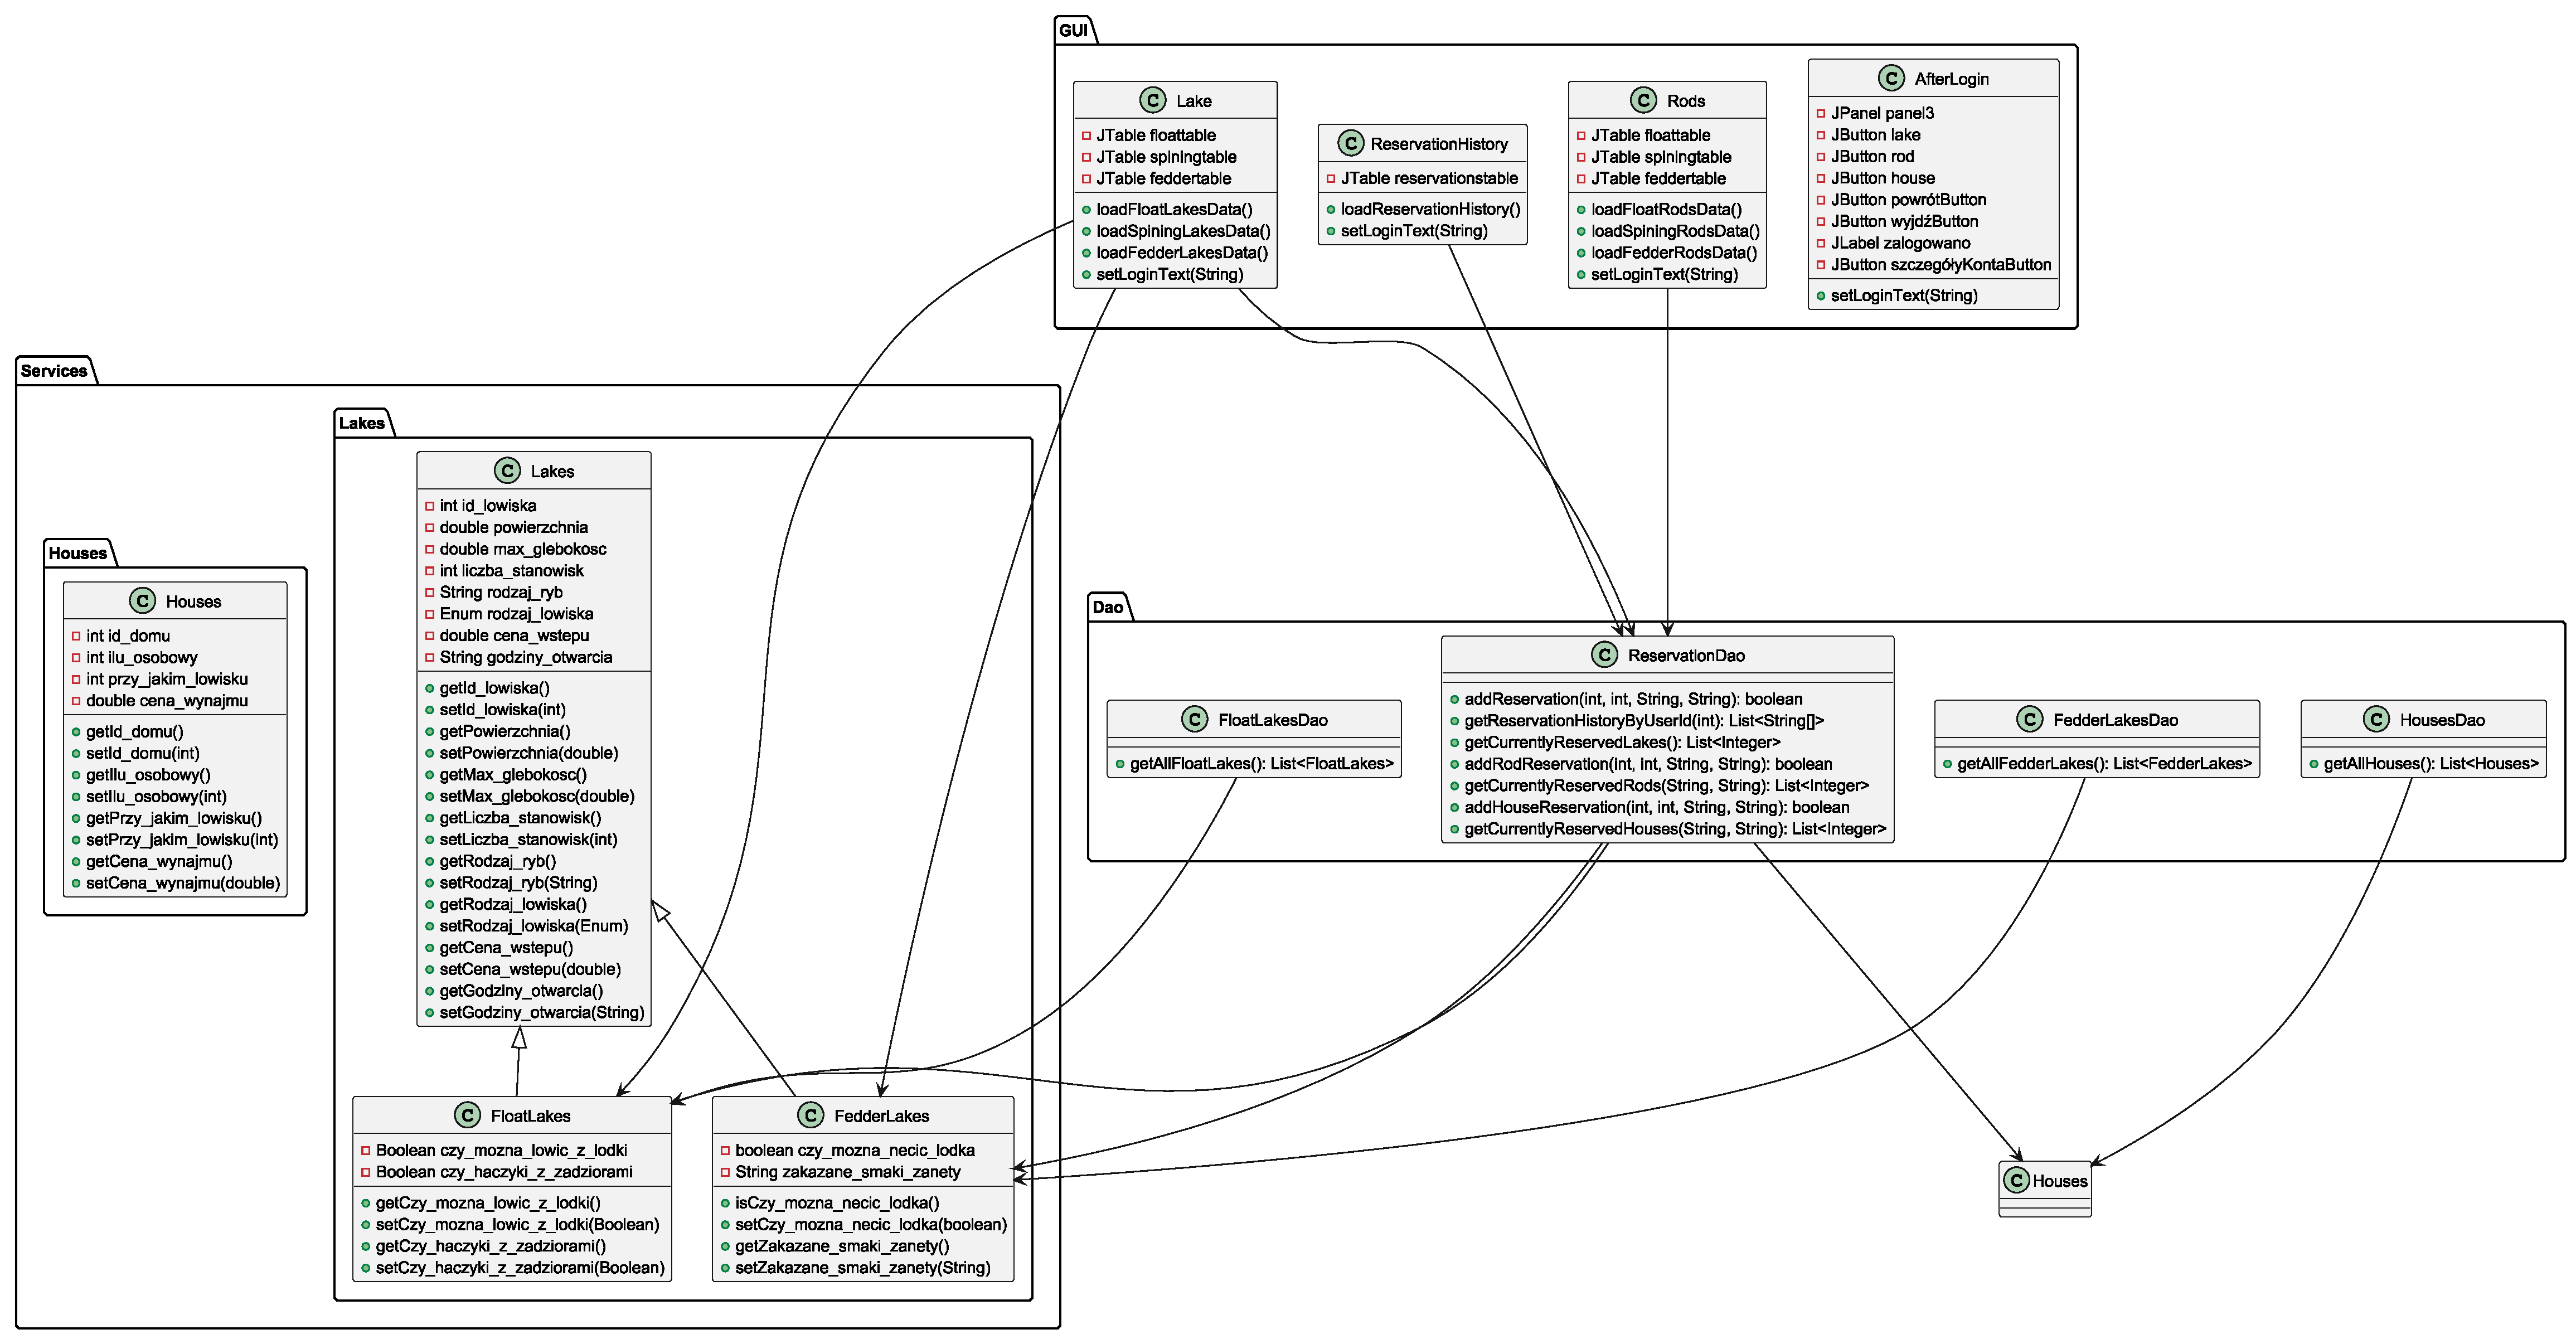
\includegraphics[width=1.1\linewidth]{figures/diagram.eps}
    \caption{Diagram klas UML projektu.}
    \label{fig:umldiagram}
    \small{Źródło: Opracowane przy użyciu PlantUML}
\end{figure}
\clearpage

\section{Zarządzanie danymi i baza danych lowisko}
\label{sec:baza_danych_nowe}
Baza danych MySQL jest kluczowym elementem projektu, przechowującym wszystkie istotne informacje o użytkownikach, rezerwacjach, łowiskach i innych zasobach. Struktura bazy danych została zaprojektowana w sposób umożliwiający łatwe zarządzanie danymi oraz ich efektywne przetwarzanie.
Baza danych składa się z kilku tabel, które są ze sobą powiązane relacjami. Główne tabele to:

\begin{figure}[H]
    \centering
    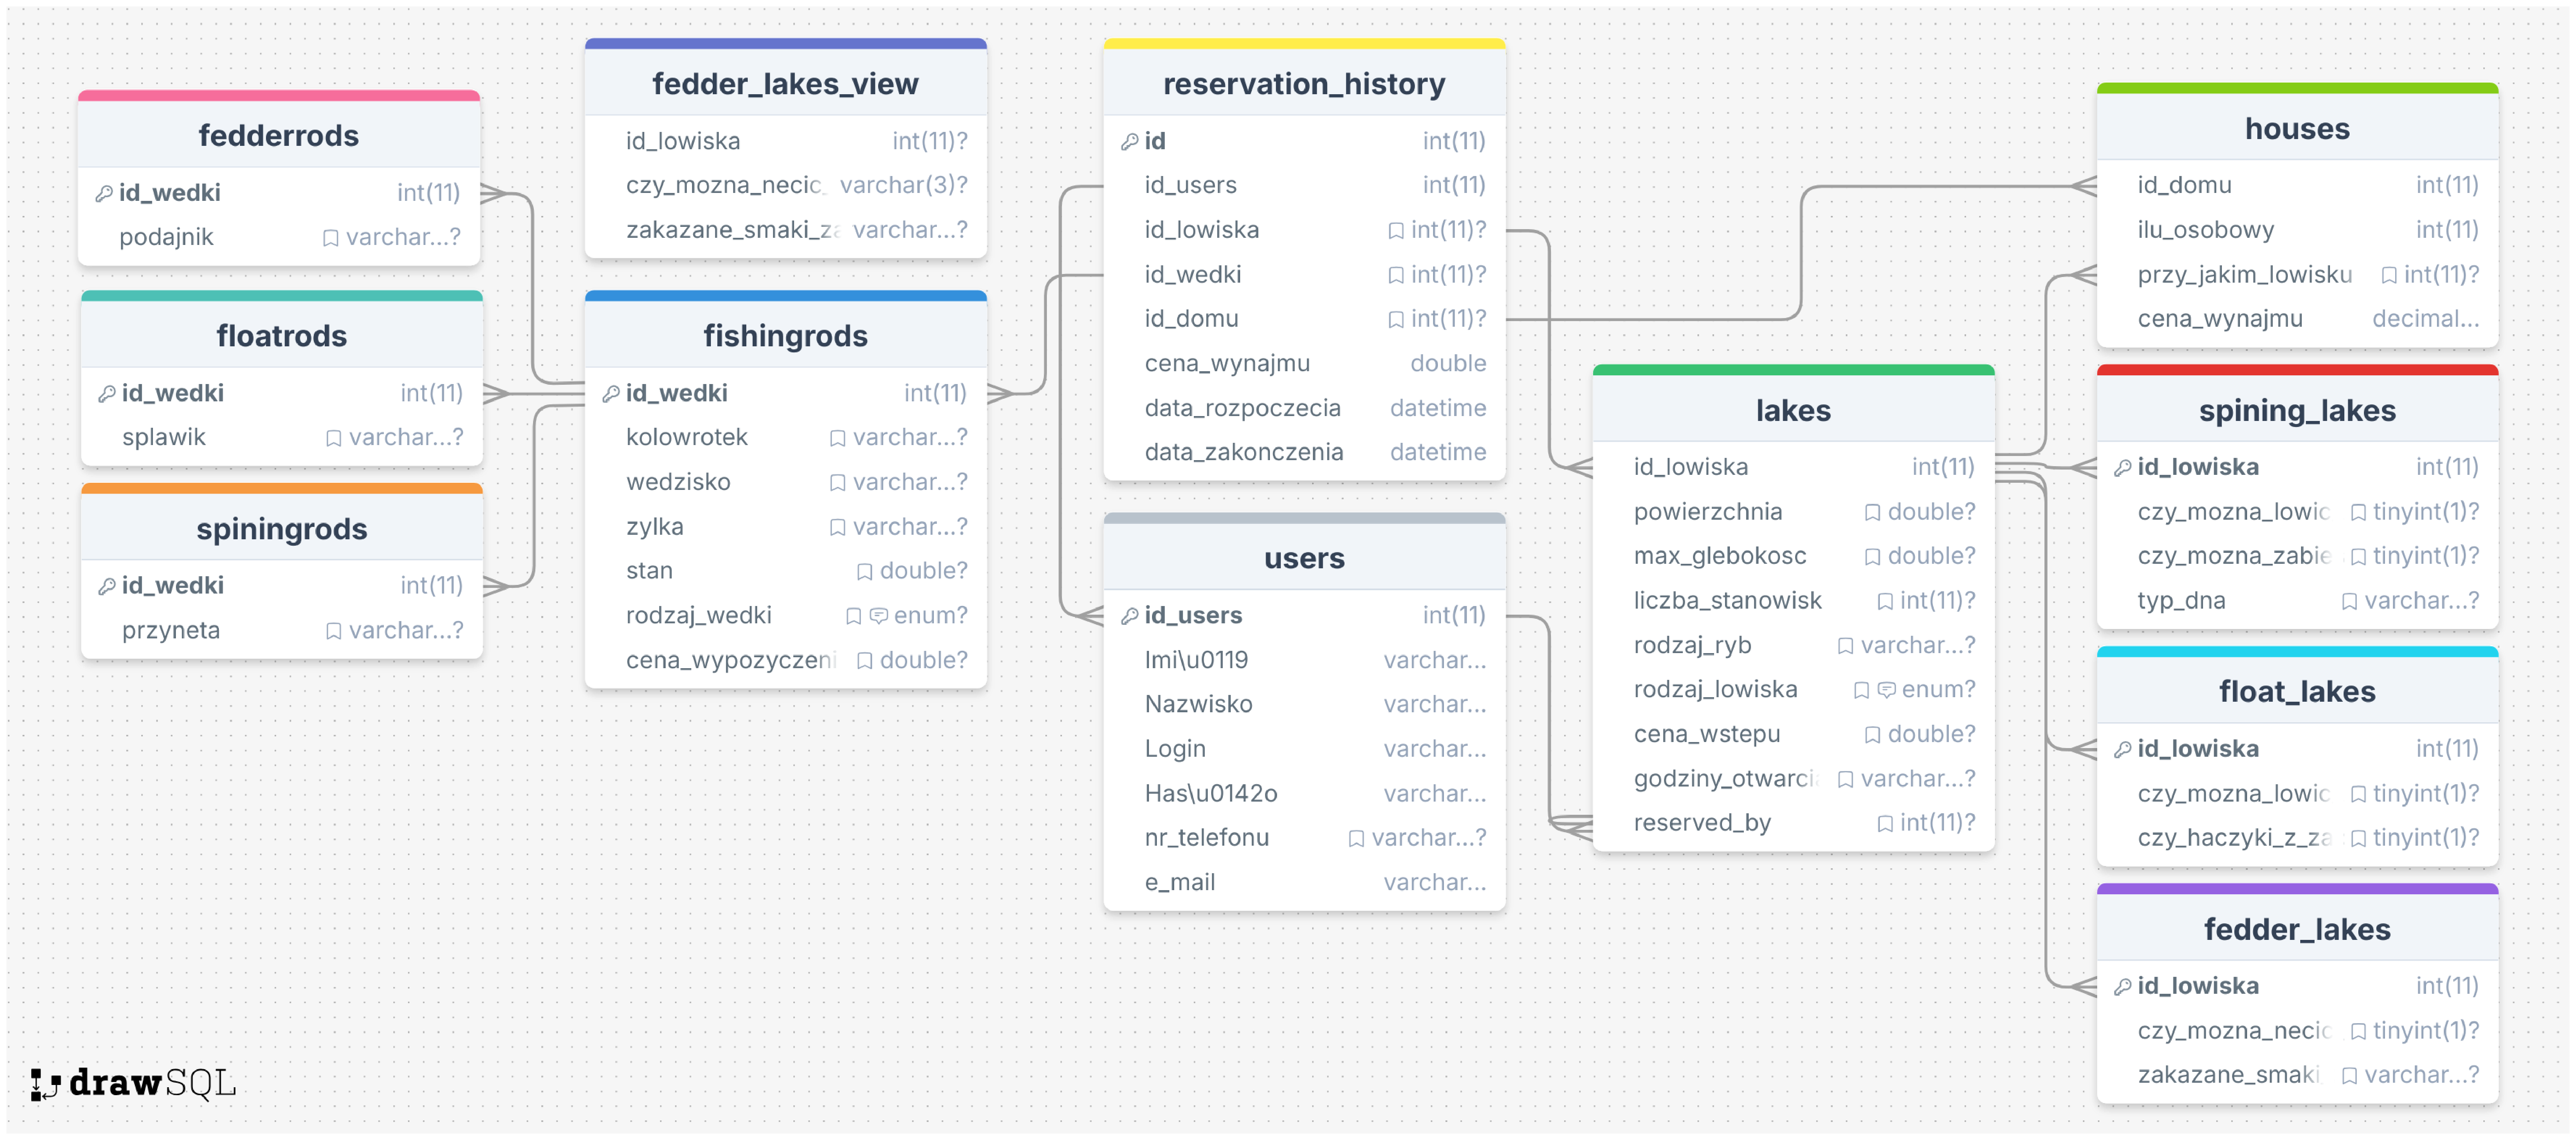
\includegraphics[width=\linewidth]{figures/dbd.eps}
    \caption{Schemat bazy danych (ERD) łowiska wędkarskiego.}
    \label{fig:erddiagram}
    \small{Źródło: Wygenerowano za pomocą https://drawsql.app}
\end{figure}
\clearpage

\section{Wymagania systemowe i narzędzia do uruchomienia projektu}
Aby uruchomić projekt, wymagane są następujące narzędzia i oprogramowanie:
\begin{itemize}
    \item \textbf{Pakiet XAMPP:} Jest to pakiet oprogramowania, który zawiera serwer Apache, MySQL oraz PHP. Jest niezbędny do uruchomienia bazy danych MySQL, która jest kluczowym elementem projektu.
    \item \textbf{Środowisko IntelliJ IDEA:} Jest to zintegrowane środowisko programistyczne (IDE) dla języka Java, w którym projekt został stworzony. IntelliJ IDEA oferuje zaawansowane funkcje, takie jak automatyczne uzupełnianie kodu, refaktoryzacja i debugowanie, co znacznie ułatwia pracę programisty. 
    \item \textbf{Java Development Kit (JDK):} Wersja JDK 17 lub nowsza jest wymagana do kompilacji i uruchomienia aplikacji. JDK zawiera wszystkie niezbędne biblioteki i narzędzia do pracy z językiem Java.
    \item \textbf{MySQL Connector/J:} Jest to sterownik JDBC dla MySQL, który umożliwia aplikacji Java komunikację z bazą danych MySQL. Należy go dodać do project structure w modułach w projekcie IntelliJ IDEA.
\end{itemize}

    


